\section{Select the client distribution}\subsection{Information:}
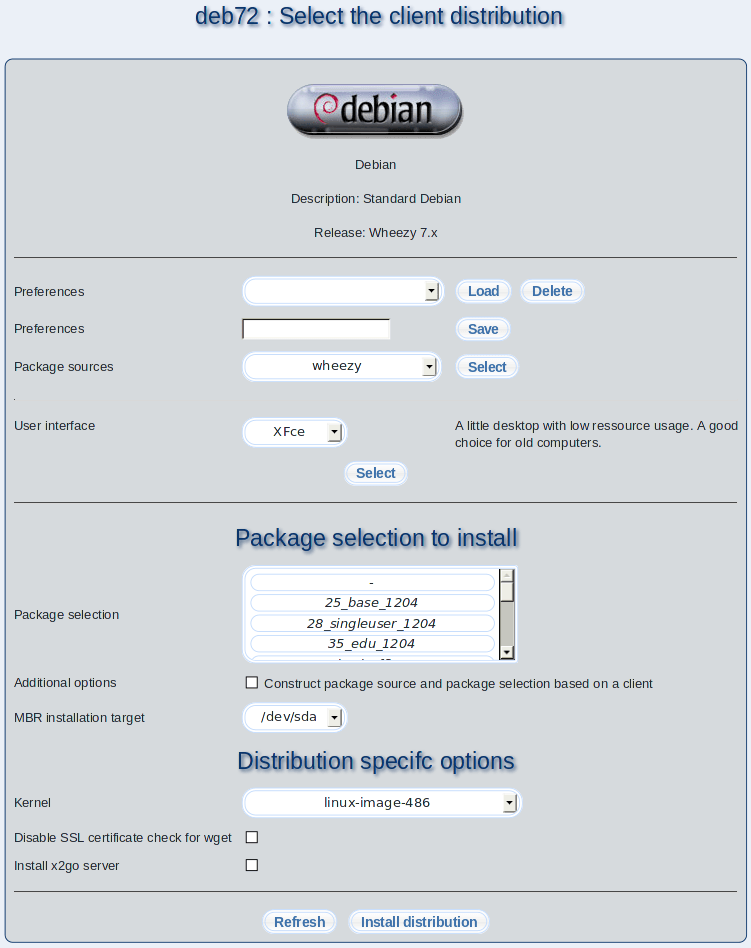
\includegraphics[scale=0.4]{/mdk/doc/manual/screenshots/en/client_distr.png} \\
A distribution is a composition of different software packages stored on CDs, DVDs or in the internet. Some of these distributions are free software and available for free download. E.g. Debian is a free Linux distribution. Distributions differentiate in the installation program and the eye candy of the desktop only. There are no significant differences. The selection of a certain distribution is mostly a matter of taste. This dialog makes it possible to install different distributions with m23.\\
\begin{itemize}
	\item \textbf{Loading preferences}: Select a previously saved preference from the list and click on \textit{"Load"}.\\
	\item \textbf{Deleting preferences}: By clicking on the \textit{"Delete"} button you can remove the selected preference.\\
	\item \textbf{Saving preferences}: You can save the current values as a preference by entering a name and clicking on the \textit{"Save"} button.\\
	\item \textbf{Package sources}: You have to choose the package source first that can be found, created or modified under  \textit{Packages} $\rightarrow$ \textit{Package sources}. Choosing a package selection predefines the Linux distribution and the distribution's release and the installable user interfaces. Click on \textit{"Select"} to choose the package source. The logo and a short descriptive text for the choosen distribution will be shown.\\
	\item \textbf{User interface}: Depending on the selected distribution, you have the choice between different graphical user interfaces (GUIs). If you want to install a server without a graphical desktop you can select \textit{"Textmode"} .\\
	\item \textbf{Package selection}: You can choose a package selection that will be installed together with the operating system.\\
	\item \textbf{MBR installation target}: m23 tries to detect the first harddisk drive for installing the bootmanager automatically. If you want to choose a different disk, you can do it here. Please keep in mind that you have to choose the drive that is the first in the BIOS booting order.\\
	\item \textbf{Distribution specifc options}: Every distribution can define a variety of options which are used during the distribution installation.\\
\end{itemize}
To start the installation simply click on \textit{"Install distribution"}.\\
\subsection{Hint for imaging}
Select \textit{"imaging"} as package sources to install images.\\
You can choose if you want to install a previously created MBR file or the generic bootloader of m23 to the the client's MBR (Master Boot Record). Select the file name or \textit{"Generic MBR"} from the \textit{"Install the generic MBR or the MBR from an image"} list.\\
\subsection{Hint:}
If you save a preference under the same name as a preference for client settings, the distribution settings will be added to the preference. On the other hand, distribution specific preferences will be overwritten.\\
